
\subsection{Dataset Overview}

To begin the analysis, I first wanted to understand the basic structure of the dataset. The dataset contains private messages exchanged on an online social network at UC Irvine. Each row represents a message with the following fields:

\begin{itemize}
    \item \texttt{SRC}: ID of the sender
    \item \texttt{TGT}: ID of the receiver
    \item \texttt{UNIXTS}: timestamp of the message in Unix time
\end{itemize}

Since UNIX timestamps are not human-readable, I converted them into datetime objects. To make the time information meaningful in the local context of UC Irvine, I also converted the times from UTC to Pacific Time (America/Los\_Angeles), accounting for daylight saving time.

\subsection{First Impressions}

I asked myself: \textit{"How big is this dataset? How many users are involved and over what time span?"}

\begin{itemize}
    \item Number of messages: 59,835
    \item Unique users: 1,899
    \item Time range: From April 15, 2004 to October 26, 2004
\end{itemize}

This confirmed that the data spans over six months and involves a sizable number of participants.

\subsection{Message Volume Over Time}

Curious about activity trends, I aggregated the number of messages sent per day. Figure~\ref{fig:messages-per-day} shows clear fluctuations, including spikes in activity that might correspond to academic events or social dynamics within the university.

\begin{figure}[H]
    \centering
    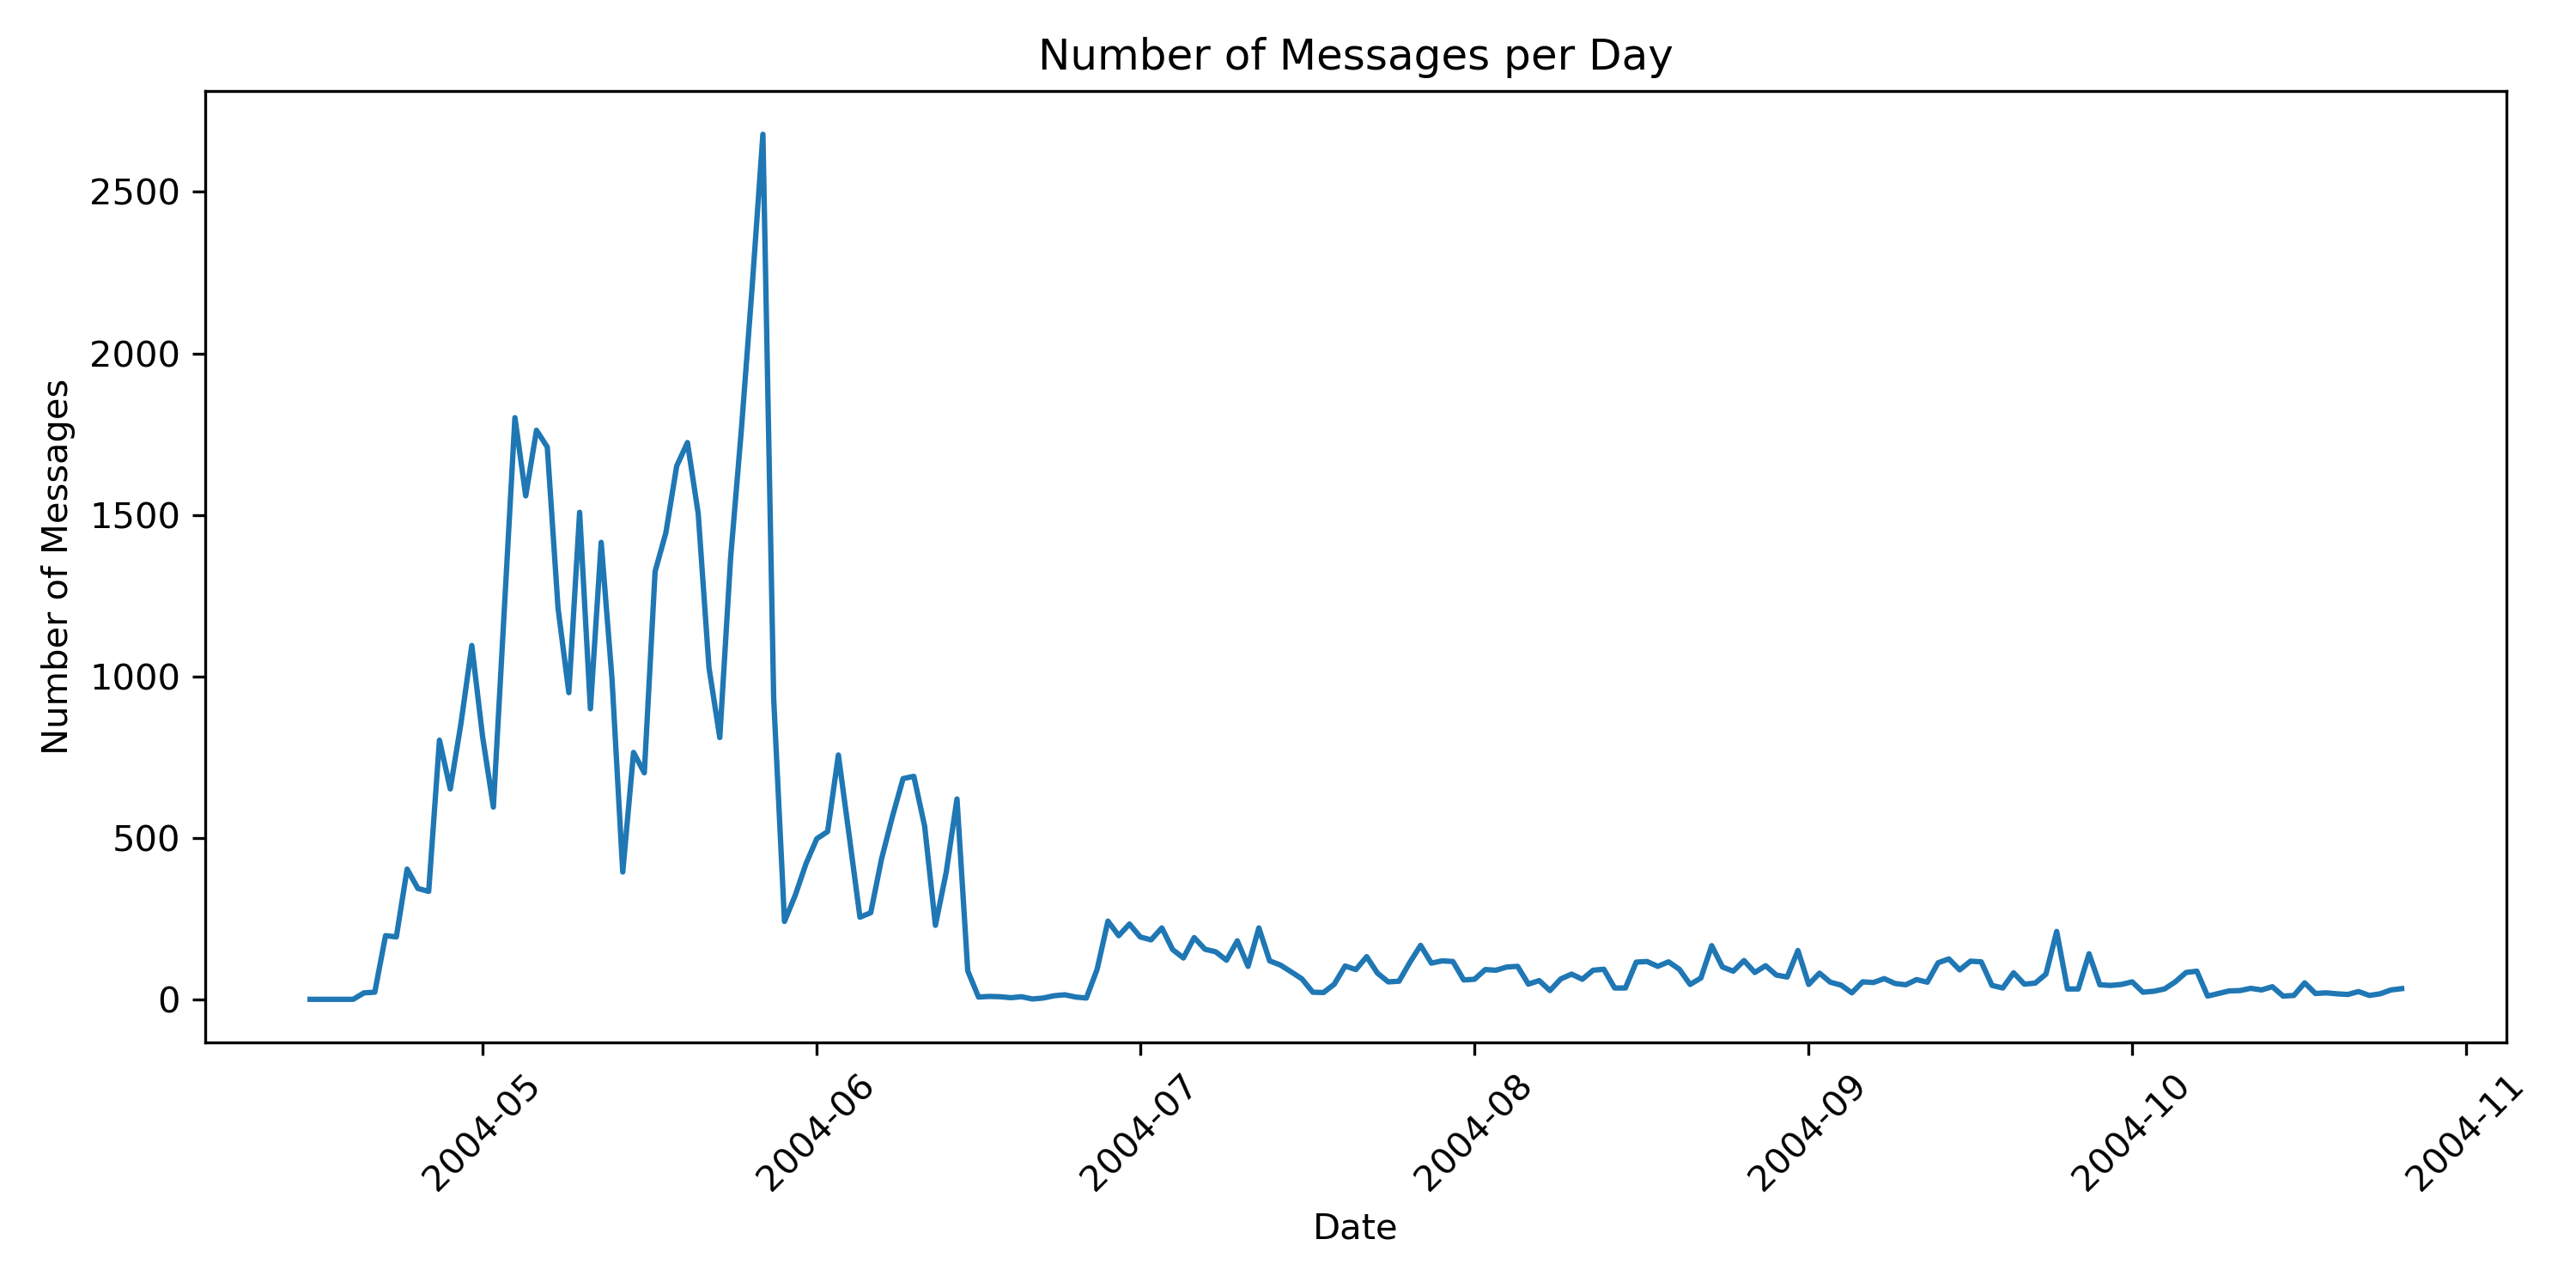
\includegraphics[width=0.4\linewidth]{../Images/messages_per_day.png}
    \caption{Daily message volume over time}
    \label{fig:messages-per-day}
\end{figure}

\subsection{Temporal Distribution by Hour, Weekday, and Month}

\subsubsection*{Messages by Hour}

Initially, I plotted the number of messages sent per hour of the day, using UTC timestamps. This produced a surprising result: a peak in activity between 5:00 and 8:00 a.m. This seemed odd for student behavior.

\textbf{Hypothesis:} The timestamps were in UTC. If users are based in California, messages should be shifted 7 hours backward.

After converting timestamps to Pacific Time, the new plot (Figure~\ref{fig:messages-by-hour}) showed a peak between 10:00 a.m. and 1:00 p.m., which is far more plausible.

\begin{figure}[H]
    \centering
    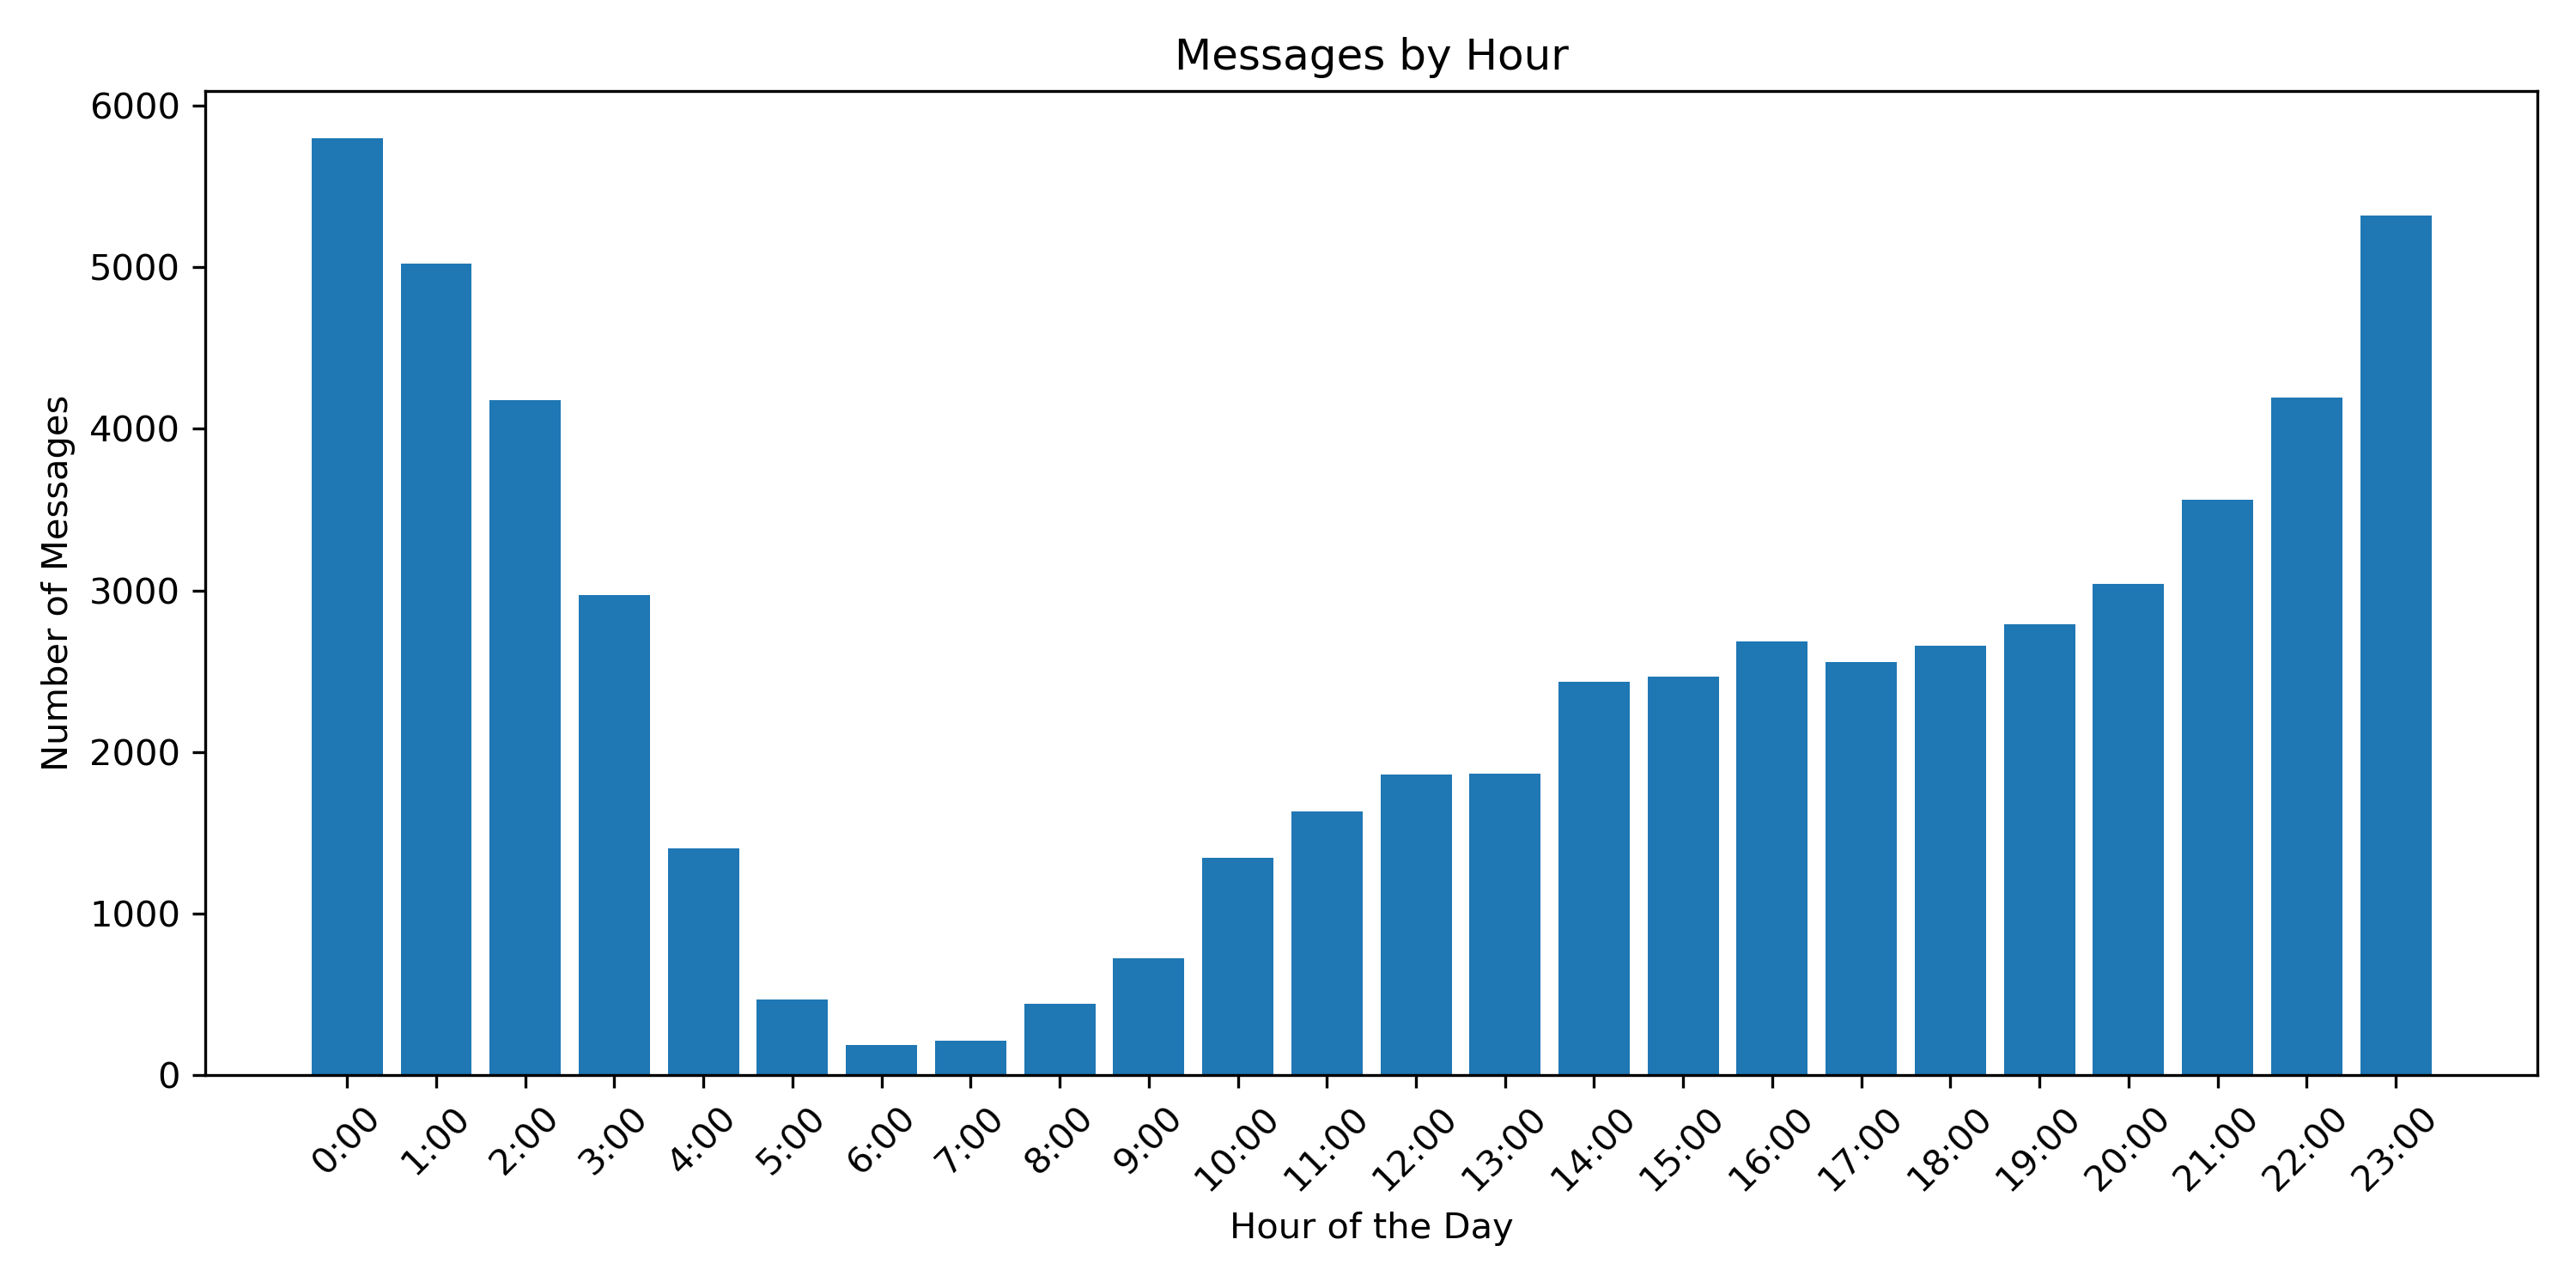
\includegraphics[width=0.3\linewidth]{../Images/messages_by_hour.png}
    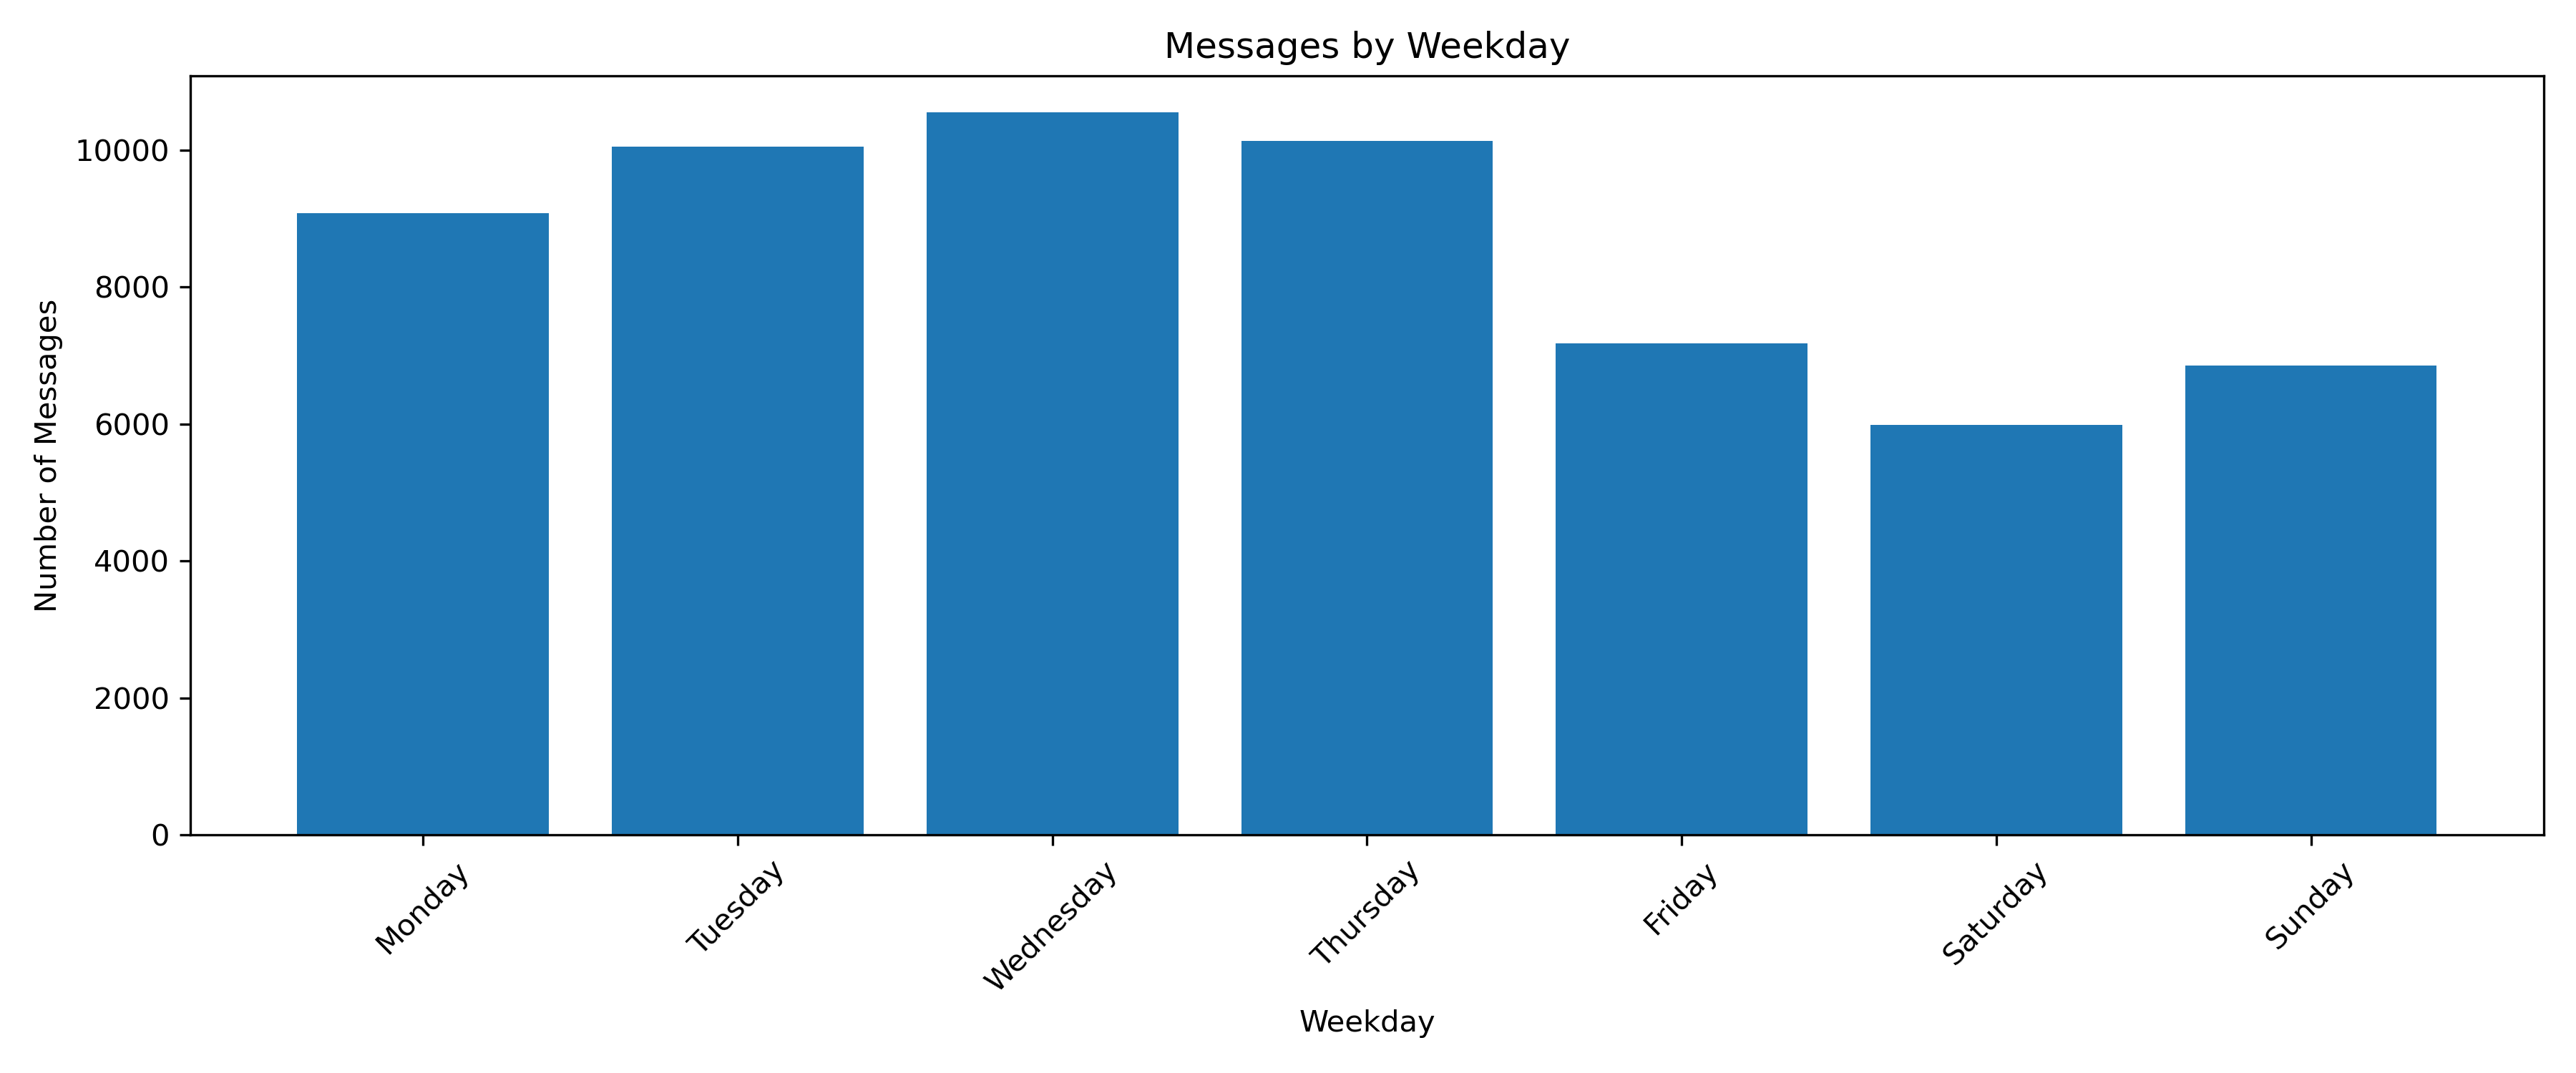
\includegraphics[width=0.3\linewidth]{../Images/messages_by_weekday.png}
    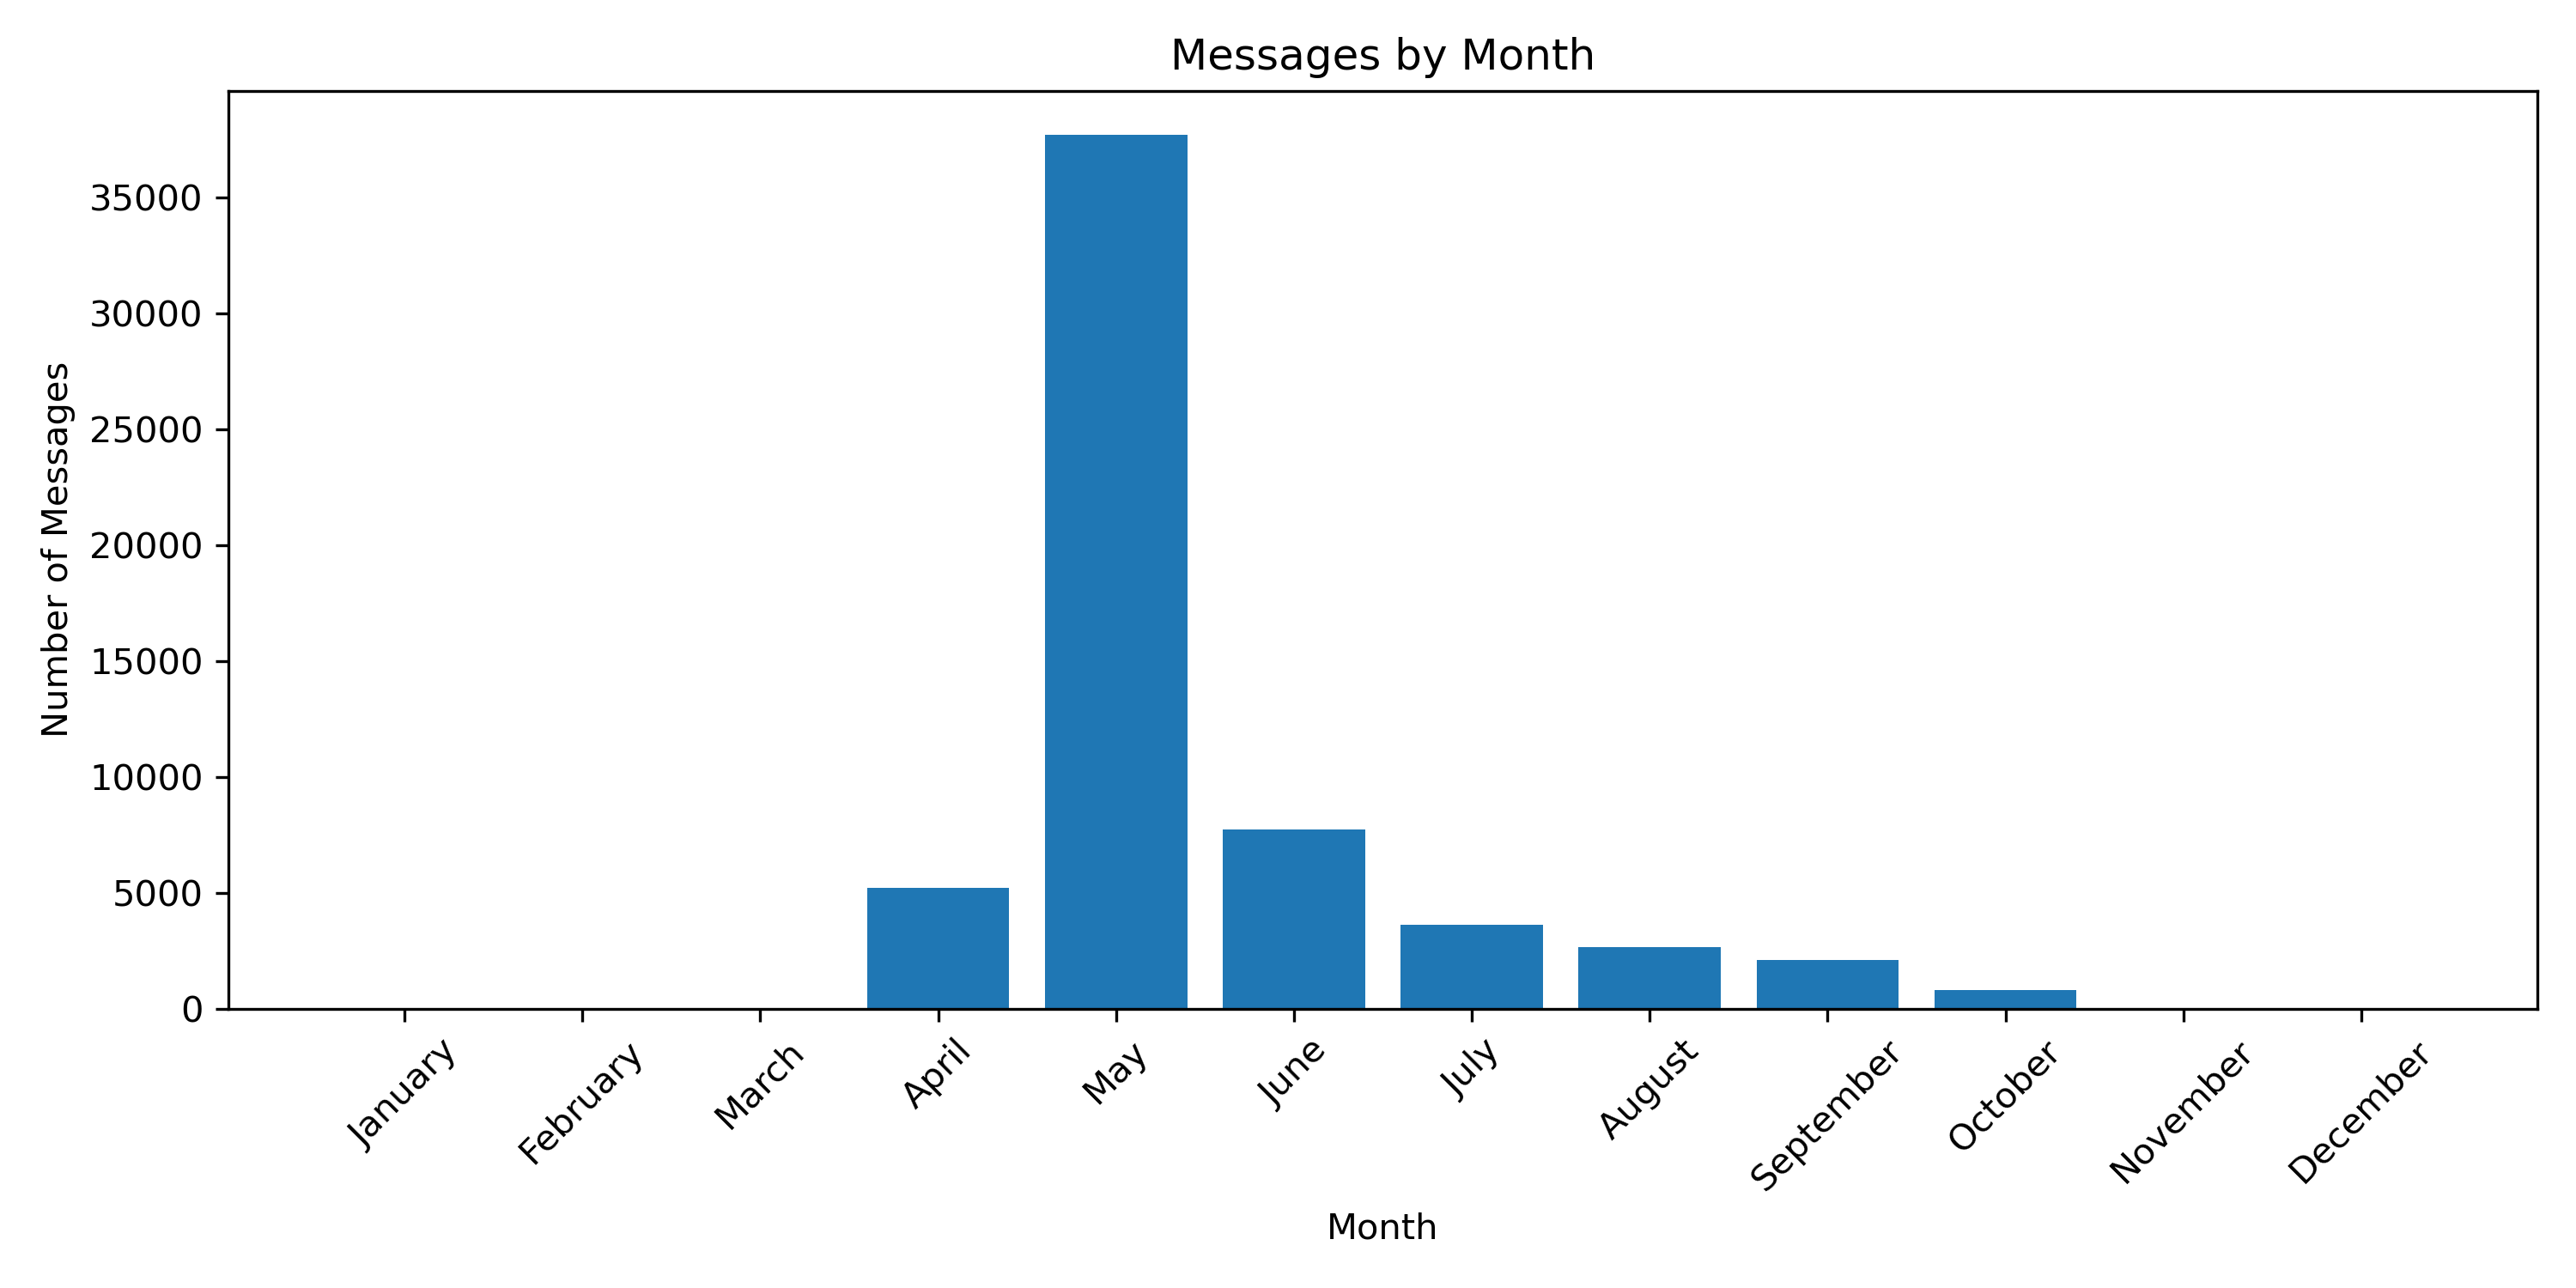
\includegraphics[width=0.3\linewidth]{../Images/messages_by_month.png}
    \caption{Messages by hour of day (after UTC to PST conversion)}
    \label{fig:messages-by-hour}
\end{figure}

\subsubsection*{Messages by Weekday}

Next, I asked: \textit{"Do students behave differently on weekdays compared to weekends?"} 

Figure~\ref{fig:messages-by-hour} reveals a drop in activity during weekends, suggesting that most messaging activity is related to academic or weekday social interactions.

\subsubsection*{Messages by Month}

Figure~\ref{fig:messages-by-hour} shows that messaging activity increased through the spring and summer months, peaking around mid-year and then tapering off.

\subsection{Network Construction}

I then asked: \textit{"How are these users connected? Can we build a graph from the data?"}

To answer this, I constructed a directed graph using the sender and receiver columns. Repeated communications between users were aggregated as weighted edges.

\begin{itemize}
    \item Nodes: 1,899
    \item Edges: 20,296
    \item Graph density: 0.0056
\end{itemize}

The graph is sparse, but this is typical in social networks where users only communicate with a small subset of others.

\subsection{User-Level Analysis: Active vs Inactive Users}

I wanted to find out: \textit{"Are there certain users who dominate the conversation? What are their behavioral patterns?"}

To address this, I computed PageRank scores to identify the most central users. I focused on User 234 as one of the most active.

\begin{figure}[H]
    \centering
    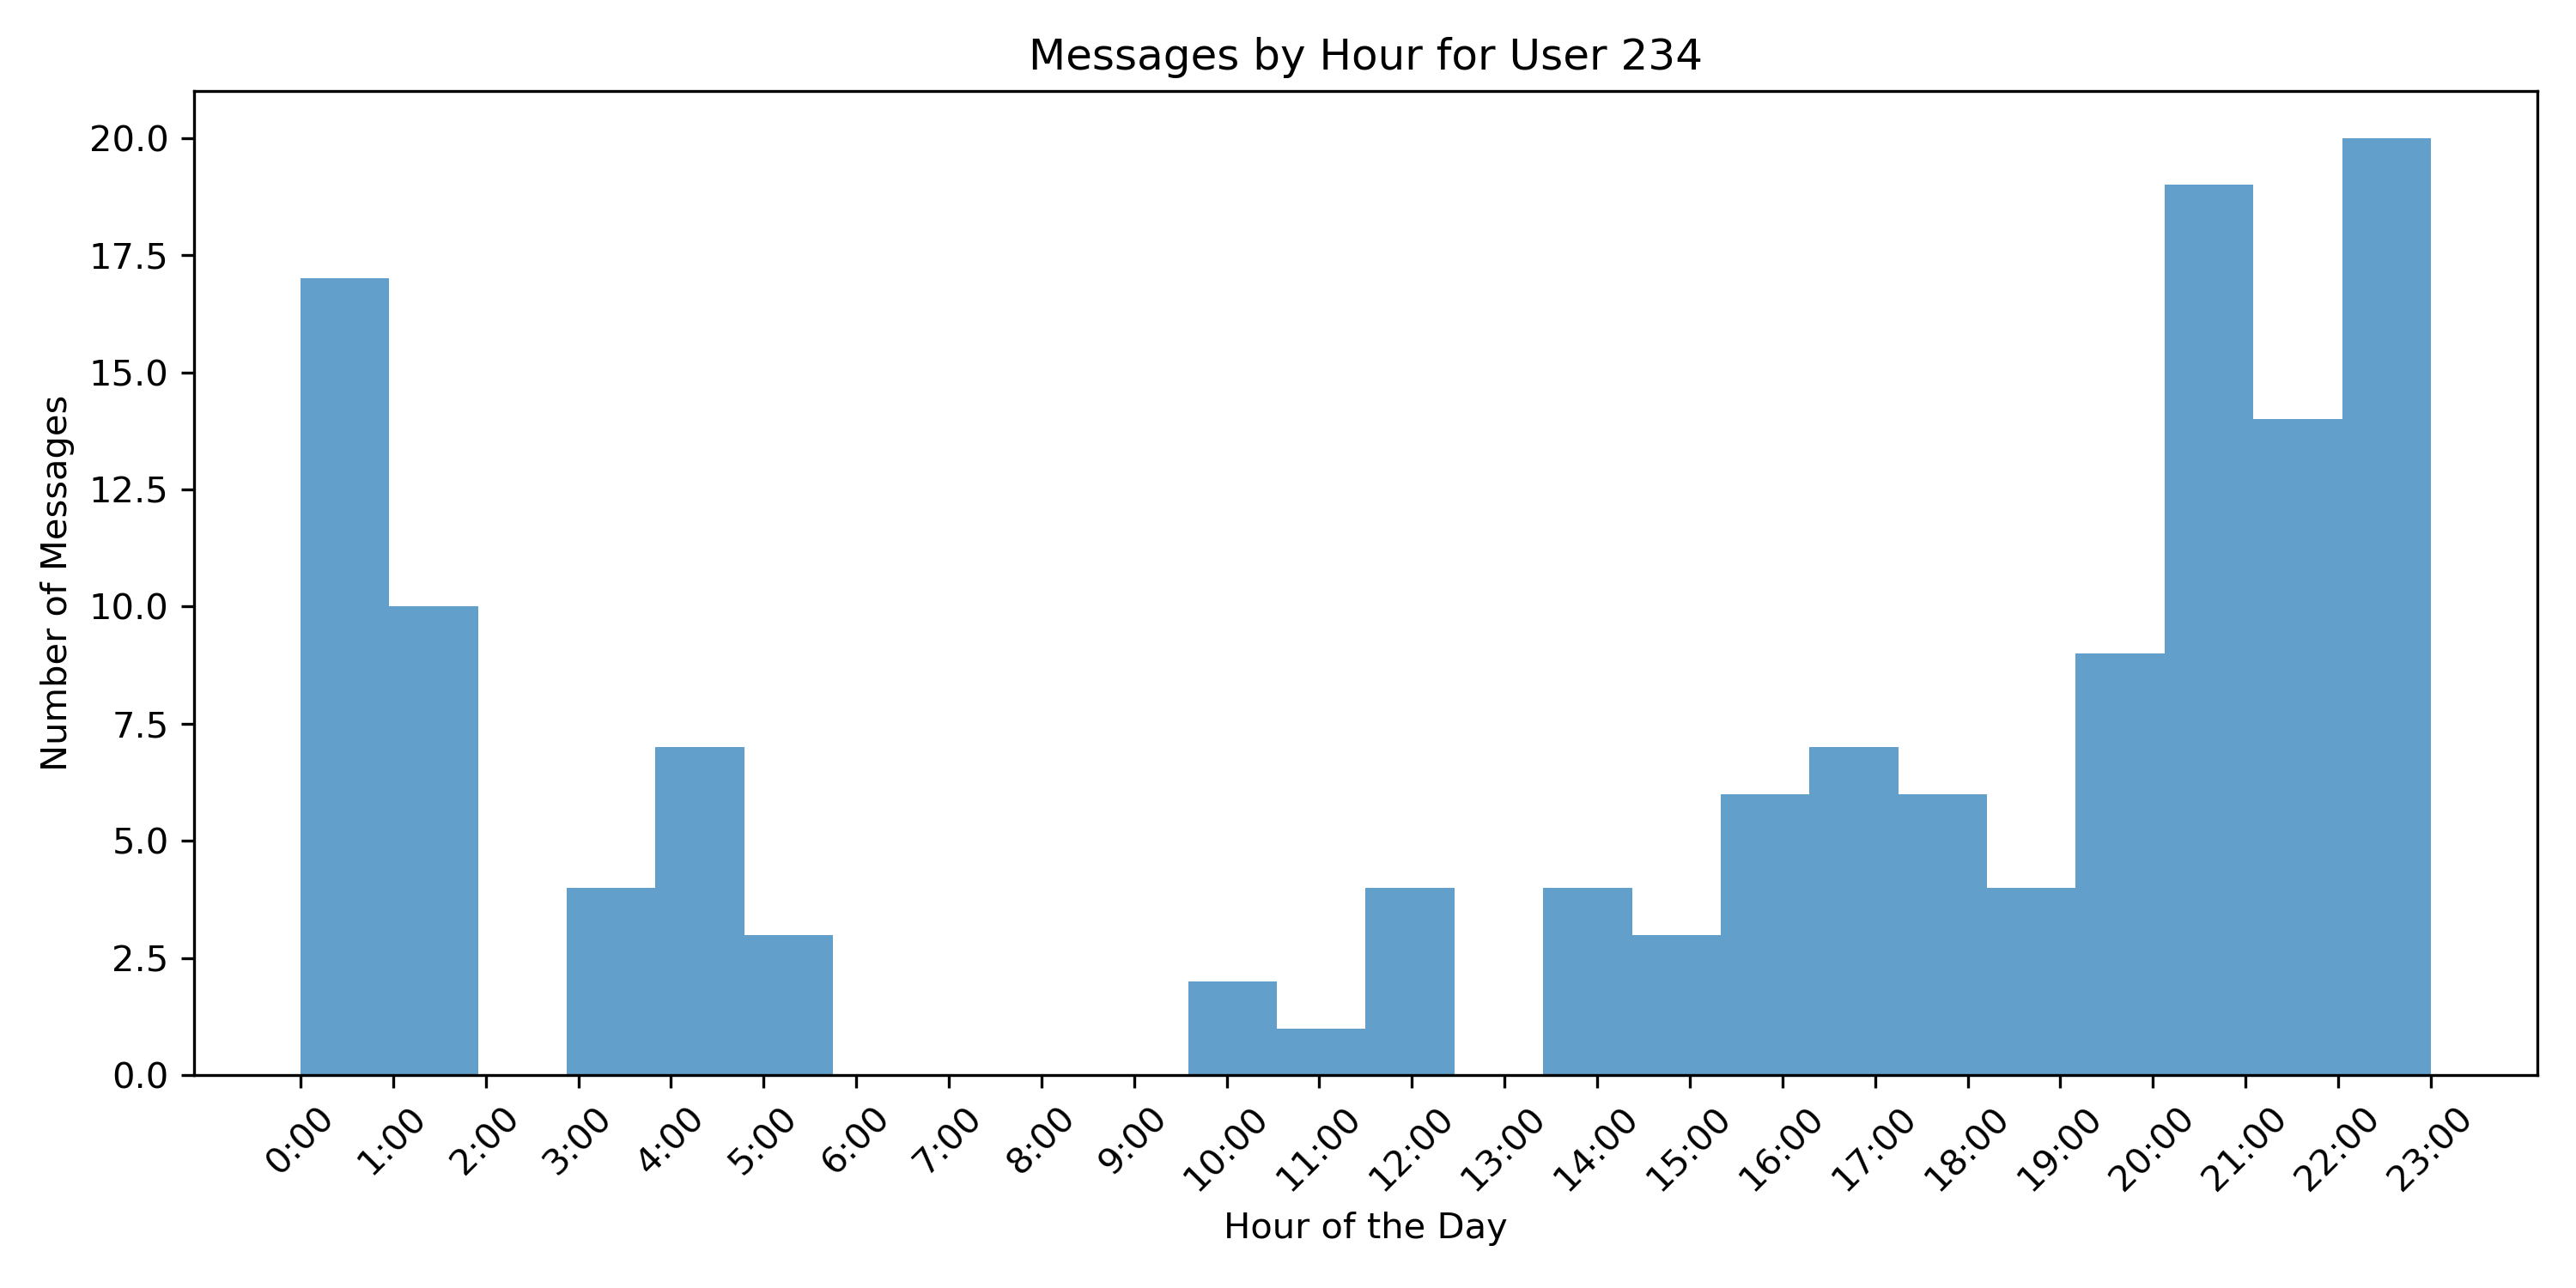
\includegraphics[width=\linewidth]{../Images/user_234_messages_by_hour.png}
    \caption{Messages by hour for User 234}
    \label{fig:user234-hourly}
\end{figure}

As seen in Figure~\ref{fig:user234-hourly}, this user was active at all hours, with a peak in the late evening.

\subsection{Comparing Central vs Peripheral Users}

Finally, I asked: \textit{"Do central users have different messaging patterns compared to peripheral users?"}

I computed the average number of messages per hour for:

\begin{itemize}
    \item The top 10 users by PageRank
    \item The bottom 1500 users by PageRank
\end{itemize}

\begin{figure}[H]
    \centering
    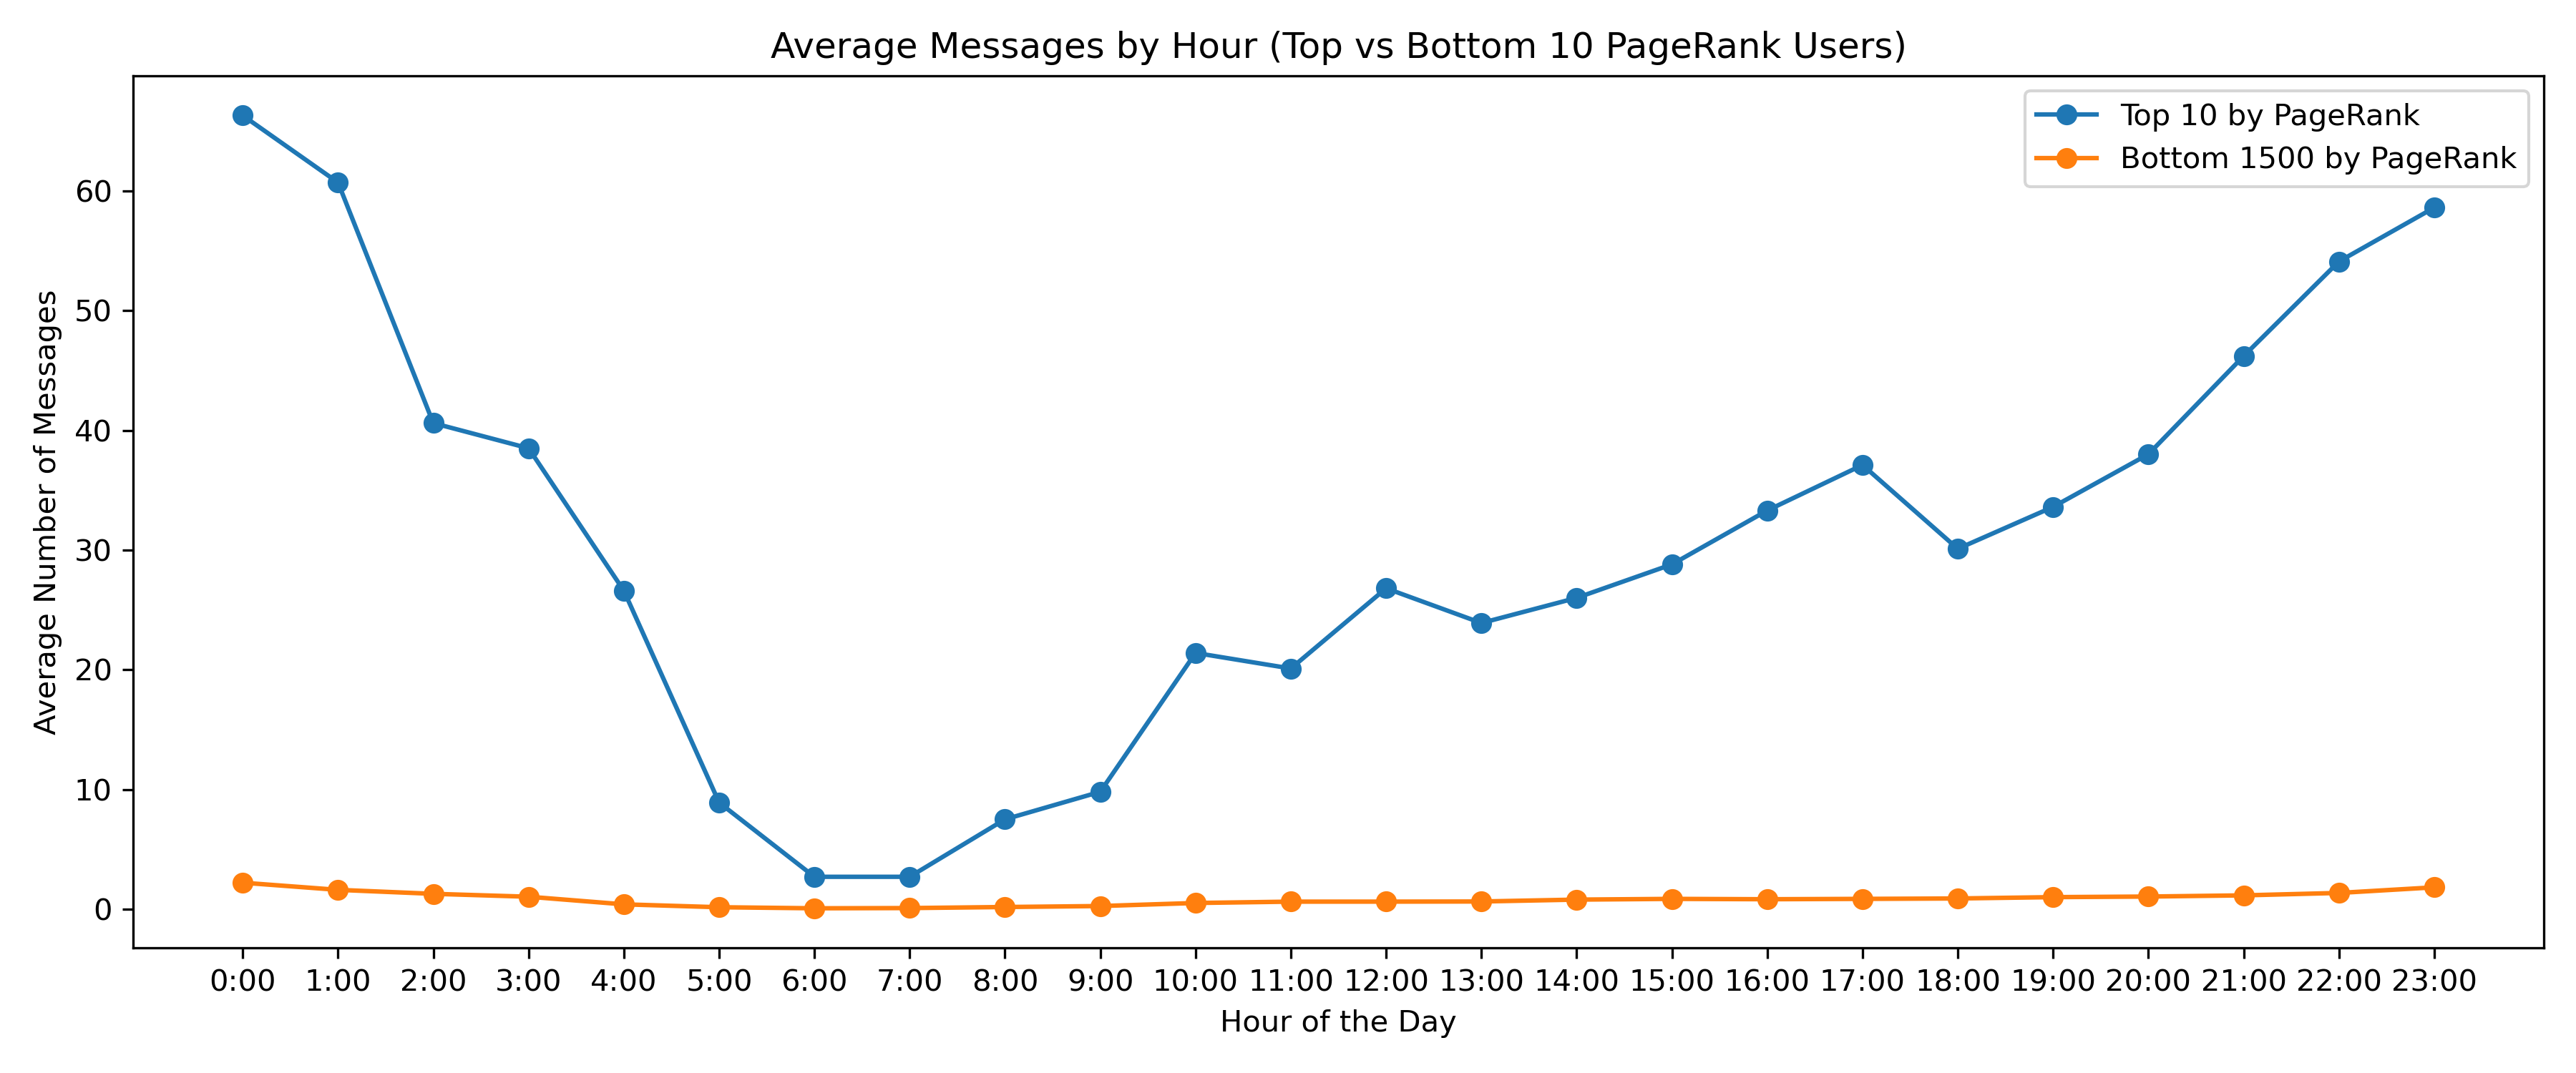
\includegraphics[width=\linewidth]{../Images/average_messages_by_hour_top_bottom.png}
    \caption{Average hourly activity: Top vs. Bottom PageRank users}
    \label{fig:top-vs-bottom}
\end{figure}

The results (Figure~\ref{fig:top-vs-bottom}) show that top users are more consistent and active throughout the day, especially during working hours, while peripheral users show sparse and inconsistent patterns.

